\section{Bottom-up block failure modeling}
\label{sec:bottom-up-modeling}

\subsection{Block failure characterization and modeling method}
\label{sec:block-failure-cz}

% What is bottom up
The modelling method presented in this section focuses first on studying low-level cells of the circuit.
They are characterized individually, leading to the definition of a failure model for each cell.
In a second step, the individual models are linked together.
The connection between the models reproduce the connections between the cells in the actual circuit.
Finally, an electrical stimulus such as an electrostatic discharge is fed on the input of the first model.
It is applied on this model that produces an output signal.
In turn, this signal is used as stimulus for the second model in the chain which is using it as input.
The process is repeated until the last output, where the output signal represents the shape of the disturbance after going through the entire chain.

% Why bottom up
The main perk of this characterization method is the modularity, because each block is characterized independently of the others.
The model built for each cell is reusable, and once the characterization is done it does not need to be repeated unless modifications are brought to the circuit.
This method is called bottom-up because low-level functions components are characterized then assembled to model higher-level functions, rising from the bottom of the hierarchy to upper levels.

% Models are not electrical but failure models
The goal of this method is to build a propagation model and not an electrical \gls{spice} model.
The models built here are not usable directly in standard simulations and does not produce strict waveforms on their ouputs.
Instead, they represent input and output waveforms by bounding boxes of a given amplitude and width.
The methodology is built on the hypothesis that simplified \gls{esd} waveforms could be sufficient to estimate the robustness of an integrated function.
This hypothesis is tested as detailed later in the document.

% Describe the changes
Several refinements of the modelling methods were applied to solve issues as they were encountered.
This chapter gives a logical history of those improvements in order to understand the starting phase and the modifications applied after.
Initially, Wunsch and Bell characterization \cite{wunsch-bell} is used to determine failure levels of individual cells when exposed to stresses of different width and amplitude.
A single failure criteria was preliminary established for each model.
It usually took the form of a voltage threshold applied on the output of a cell, above which a fault is recorded.
This treshold is set prior to the simulation, and there is no general rule for setting it.
The \gls{dc} specification of the output can be used directly, if it exists, or a sound value in regard of the design, or an arbitrary level.

% How is it done, core concept
The first part of the modelling method is the characterization of each block using the electrical setup of Fig. \ref{block_function_cz} in a \gls{spice} simulation environment.
This setup provides appropriate biasing to the block with V\textsubscript{DC} voltage source, in order to set the block function in operating conditions.
It also enables the injection of the characterization signal on the tested input with V\textsubscript{stress} transient voltage source.
The characterization pulses are rectangular waveforms similarly to the Wunsch and Bell technique.
Each simulation runs with a different pair of values for the \textbf{amplitude} and \textbf{duration} of the square signal.
On the other side of the cell under test, the output is monitored.
Prior to the simulation, a failure criteria consisting of a voltage threshold is set.
If the output waveform goes above this threshold, the simulation is tagged as \textit{fail}.
The threshold is chosen depending on multiple parameters such as the functionality of the block or its DC operating point.

\begin{figure}[!h]
  \centering
  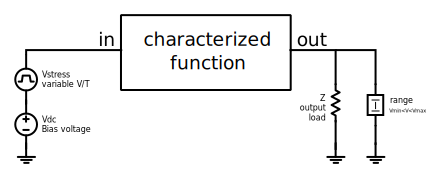
\includegraphics{src/4/figures/characterization_setup.pdf}
  \caption{Block characterization setup (supply input)}
  \label{block_function_cz}
\end{figure}

The results are summarized into table \ref{simulation-results}.
The simulations in red contain a fail, meaning that the output voltage crossed the failure threshold.

\begin{table}[!h]
\centering
\begin{tabular}{@{}lllll@{}}
\toprule
    & 1ns                          & 10ns                         & 100ns                        & 1\textmugreek{}s             \\ \midrule
15V & {\color[HTML]{FE0000} sim13} & {\color[HTML]{FE0000} sim23} & {\color[HTML]{FE0000} sim33} & {\color[HTML]{FE0000} sim43} \\
10V & {\color[HTML]{32CB00} sim12} & {\color[HTML]{FE0000} sim22} & {\color[HTML]{FE0000} sim32} & {\color[HTML]{FE0000} sim42} \\
5V  & {\color[HTML]{32CB00} sim11} & {\color[HTML]{32CB00} sim21} & {\color[HTML]{32CB00} sim31} & {\color[HTML]{FE0000} sim41} \\
\bottomrule
\end{tabular}
\caption{Example of results on a set of simulations}
\label{simulation-results}
\end{table}

% A first visualization of the characterization
A curve can be built from this table to give a visual representation of the functional robustness of the block (see Fig. \ref{wb_cz_curve_example}).
The x axis is the duration of the input stress.
The y axis is the amplitude of the input signal during the stress.
The color of the curve (red or green) corresponds to the presence or absence of failure at the given input amplitude and width.

\begin{figure}[!h]
  \centering
  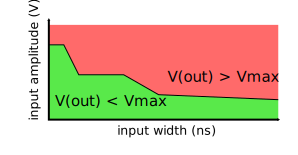
\includegraphics{src/4/figures/example_curve.pdf}
  \caption{Visual representation of powered-on block testing results}
  \label{wb_cz_curve_example}
\end{figure}

% How to improve the displayed information
Presence or absence of a failure is not the only information that can be obtained by monitoring the output.
Because soft-failures are temporary issues, their duration is also very relevant.
Using the same characterization setup as before (Fig. \ref{block_function_cz}), it is possible to also measure the duration of a failure.
It is possible to improve table \ref{simulation-results} by replacing the fail or no-fail flag by the duration of the fail.
This is illustrated in table \ref{simulation-results-bis}.
With those example values, for an input pulse stress of 5V with a input pulse width of 1ns, no failure was recorded.
On the other hand, with a 5V 1\textmu{}s stress, a failure was recorded and the output waveform crossed the threshold during 2\textmu{}s.
A 15V 1\textmu{}s stress caused a failure that lasted 30\textmu{}s.

\begin{table}[!h]
\centering
\begin{tabular}{@{}lcccc@{}}
\toprule
    & \multicolumn{1}{l}{1ns}      & \multicolumn{1}{l}{10ns}     & \multicolumn{1}{l}{100ns}    & \multicolumn{1}{l}{1us}     \\ \midrule
15V & {\color[HTML]{00D2CB} 110ns} & {\color[HTML]{FFCB2F} 150ns} & {\color[HTML]{FE0000} 30us}  & {\color[HTML]{FE0000} 30us} \\
10V & {\color[HTML]{32CB00} }      & {\color[HTML]{00D2CB} 125ns} & {\color[HTML]{F8A102} 540ns} & {\color[HTML]{FE0000} 30us} \\
5V  & {\color[HTML]{32CB00} }      & {\color[HTML]{32CB00} }      & {\color[HTML]{32CB00} }      & {\color[HTML]{F56B00} 2us}  \\
\bottomrule
\end{tabular}
\caption{Example result set containing failure width information}
\label{simulation-results-bis}
\end{table}

% How to improve the curve from the improved table
This improvement can also be transfered to the curve representation.
A gradient is used rather than a fail or no-fail area.
The gradient color for each location corresponds to the failure duration the output.
The figure \ref{wb_cz_curve_example_v2} provides an example of this improved representation.
In this figure, the warmer the gradient, the longer the output is disturbed.

\begin{figure}[!h]
  \centering
  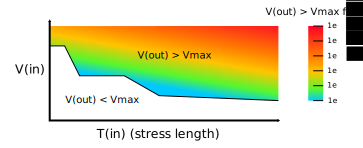
\includegraphics{src/4/figures/example_curve_v2.pdf}
  \caption{Improved curve for Wunsch and Bell powered-on characterization}
  \label{wb_cz_curve_example_v2}
\end{figure}

The gradient can also be discretized into a few aeras for better readability as shown in figure \ref{wb_cz_curve_example_v2_discrete}.
This representation looses some information compared to the gradient one, but is easier to generate and read.

\begin{figure}[!h]
  \centering
  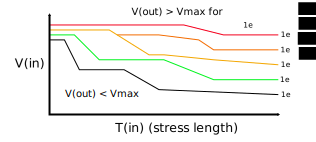
\includegraphics{src/4/figures/example_curve_v2_discrete.pdf}
  \caption{Improved discrete curve for Wunsch and Bell powered-on characterization}
  \label{wb_cz_curve_example_v2_discrete}
\end{figure}

% TODO Review
% Summarize the method
Detailled a method to extract the robustness of a block function in a behavioral manner.
Inject pulses on an input and watch for changes on an output.
The block model is composed of a characterization table and a failure criteria.
It can be summarized in Fig. \ref{fig:principle-transfert-func}.
Table accepts input width and amplitude, and returns output width.
The failure criteria serves two purposes.
It is used during characterization.
It is also used as output amplitude in the next section where models are chained.

\begin{figure}[!h]
  \centering
  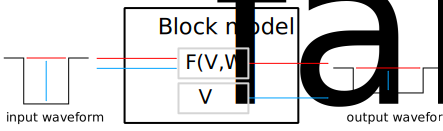
\includegraphics{src/4/figures/principle_transfert_function.pdf}
  \caption{First modelling method}
  \label{fig:principle-transfert-func}
\end{figure}

% Why modelling individual blocks
The motivation for modelling blocks individually is that a single block can be failing but the error can remain internal.
Complete function can continue to operate without changes.
In the other way around, not all blocks need to be failing in order to cause the complete function to fail as well.
It is important to determine which blocks may be in fault to be able to fix the problem.
This is why the characterization method presented here focuses on blocks and not complete functions.

% What is done next
In the next section, those individual block models are chained together to deduce the robustness of a complete function.
The processed is explained in detailed and is later applied on a practical case.

\subsection{Block models chaining}
\label{sec:block-chaining}

% Explain the chaining mechanism
The characterization process detailed previously (in \ref{sec:block-failure-cz}) is repeated on each block constituting a high-level function.
Once done, the bottom-up study now focuses on a higher level in the design hierarchy.
As a remainder, the original goal of this method is to see if the robustness of a high-level function is the sum of its parts' robustness.

Thus, individual models are connected together, by following exactly how blocks are connected in the design.
To illustrate this idea, fig. \ref{example_toplevel_function} represents an example of a high-level function, constituted of three blocks at the second level of hierarchy.
It is assumed that each of these blocks has been characterized.

% WHICH NET IS TOP MONITORED ?

\begin{figure}[!h]
  \centering
  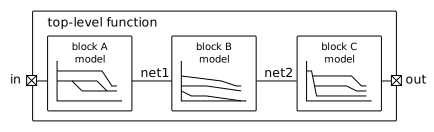
\includegraphics{src/4/figures/example_top_level_function.pdf}
  \caption{Example of a top-level function with 3 characterized blocks}
  \label{example_toplevel_function}
\end{figure}

% Remind the final goal
Now, we want to obtain the robustness of the entire function, against a given stress, using the block models.
The stress is injected on the global pin \textbf{\textit{in}}.

% What is the input stress ? What is the top-level function evaluated against ?
In this example, we will consider the stress is generated by a \gls{tlp} generator, and is thus rectangular.
For this example, the stress is chosen to have a duration of 100 ns, and an amplitude of 10V.

% How is used the characterization of the output of A on the input of B ?
%TODO: Detail a lot more. This is key. Speak about modeling of the output, and simplification to square pulse.
%TODO: Make a figure to show how is the disturbance on the output of A is modeled
The stress is injected on the global \textbf{\textit{in}} pin.
This pin is also the input pin of the first block.
Thus, the properties of the \gls{tlp} pulse can directly be applied to the model of block A.
Fig. \ref{example_complete_curve} shows an example curve for model A, and the location of the TLP pulse characteristics on this curve.

\begin{figure}[!h]
  \centering
  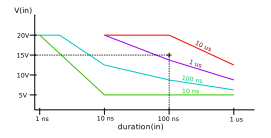
\includegraphics{src/4/figures/example_complete_curve.pdf}
  \caption{Model A curve and determination of impact of the TLP pulse - values in color represent the duration of failure on the output}
  \label{example_complete_curve}
\end{figure}

% Interpretate stress to deduce net1
Like stated earlier, the pulse has a duration of 100ns and an amplitude of 15V. By reporting this point on curve \ref{example_complete_curve},
it is visible that this will cause the output of block A to violate its failure criteria between 1 \textmugreek{}s and 10 \textmugreek{}s.
We consider, for the sake of this example, the failure criteria of block A to be net1 > 5V.
With a 100ns long 15V pulse on the input of A, the characterization states that the output of block A will go above 5V for at least 1us.
This is the best case value for net1.

% Use net1 as input of next block
\textit{net1} is the output of block A, but it is also the input of block B.
Thus, best case (amplitude, duration) values for net1 can be used as input for block B's model.
Fig. \ref{example_complete_curve_B} shows an example curve for model B, and the location of the \textit{net1} disturbance on this curve.
This shows that \textit{net2}, the output of block B and the input of block C, will go below B's failure level for at least 10 \textmugreek{}s.

\begin{figure}[!h]
  \centering
  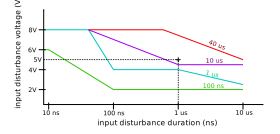
\includegraphics{src/4/figures/example_complete_curve_B.pdf}
  \caption{Model B curve and determination of impact of the TLP pulse}
  \label{example_complete_curve_B}
\end{figure}

% Repeatable process
As shown, this process can be repeated in theory with as many blocks as required by the original design, until the final pin is reached.
The is possible because the output of a block is used as the input of the next one.

%TODO: Algorithm organigram

% How to select pins to characterize

% Show how it can help to speedup and simplify the computation of the entire function robustness
